\documentclass{standalone}
\usepackage{pgf}
\usepackage{amsmath}
\usepackage{tikz}
\usetikzlibrary{shapes,arrows}
\usetikzlibrary{positioning}
\usepackage{tikz}
\usetikzlibrary{positioning}
\usetikzlibrary{shapes.geometric}
\usetikzlibrary{shapes.misc}
\usepackage{amsmath}
\usepackage{amssymb}
\usepackage{xstring}

\begin{document}
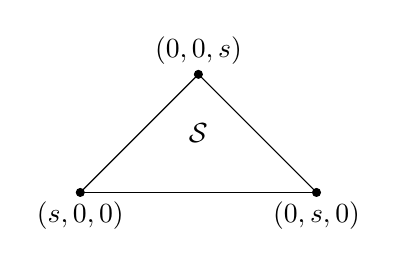
\begin{tikzpicture}
 \draw (0,0) -- (3,0);
 \draw (0,0) -- (1.5,1.5);
 \draw (3,0) -- (1.5,1.5); 

 \draw [fill=black] (0,-0.) circle (0.05) node[below, black]{${\small (s,0,0)}$};
  \draw [fill=black] (3,-0.) circle (0.05) node[below, black]{$(0,s,0)$};
 \draw [fill=black] (1.5,1.5) circle (0.05) node[above, black]{$(0,0,s)$};
 
  \draw (1.5,1) node[anchor=north] {$\mathcal{S}$};    

 \end{tikzpicture}
\end{document}} 
 %\end{document}
